\documentclass[a4paper]{article}

\usepackage[utf8]{inputenc}
\usepackage{a4wide}
\usepackage{relsize}
\usepackage{indentfirst}
\usepackage{minted}
\usepackage{graphicx}
\usepackage{float}
\usepackage{amsmath, amssymb, amsfonts, amsthm}
\usepackage{hyperref}
\usepackage[capitalise]{cleveref}
\usepackage[toc, page]{appendix}

\AtBeginEnvironment{minted}{\let\itshape\relax}

\begin{document}

\section*{Exercise 1}

See \cref{fig:dhparam}.

\section*{Exercise 2}

See \Cref{fig:dsa-prime,fig:dsa-generator}.

\section*{Exercise 3}

Without the \texttt{dsaparam} option, the generation of DH parameters takes much longer because it
generates a \textit{strong prime}, \textit{i.e.} a prime number $p$ such that $(p-1)/2$ is also prime.
This ensures that the multiplicative group $\mathbb{Z}_p^\ast$ does not contain small subgroups. The
existence of small subgroups within a larger group in a cryptographic protocol is undesirable in the
sense that it confines shared secrets to a smaller set of possible values than if it were to use the
whole group $\mathbb{Z}_p^\ast$. 

On the other hand, using the \texttt{dsaparam} DSA rather than DH parameters are read or generate, which
are then they are converted to DH format, making the key exchange process more efficient.

\vspace{\baselineskip}

\textbf{Note:} See \cref{fig:sage-dh,fig:sage-dsa}.

\section*{Exercise 4}

Running the following function with the previously generated DH parameters, we can see that
$X^y \ (\mathrm{mod} \ p) = Y^x \ (\mathrm{mod} \ p)$ holds.

\vspace{\baselineskip}

\begin{minted}{py}
from sage.all import *

def ex4(p, q):
    x = randrange(q)
    y = randrange(q)

    X = Mod(q ** x, p)
    Y = Mod(q ** y, p)

    return Mod(X ** y, p) == Mod(Y ** x, p)
\end{minted}

\vspace{\baselineskip}

\textbf{Note:} See \cref{fig:ex4-dhparam,fig:ex4-dsa}.

\section*{Exercise 5}

We know that $p = 1373, g = 2, X = 974$ and $y = 871$. We can determine $Y$ by computing the
following:

\[
Y = g^y \ \mathrm{mod} \ p = 2^{871} \ \mathrm{mod} \ 1373 = 805
\]

Knowing the value of $X$ and $y$, we can then determine the shared secret $g^{xy}$ by computing
the following:

\[
g^{xy} = (g^x)^y = X ^ y = 974 ^ {871} \ \mathrm{mod} \ 1373 = 397
\]

\pagebreak

Finally, we can find Alice's secret exponent by solving:

\[
X = g^x \ \mathrm{mod} \ p \Leftrightarrow 974 = 2^x \ \mathrm{mod} \ 1373 \Leftrightarrow x = 587
\]

\section*{Exercise 6}

The Computational Diffie-Hellman Problem (CHD) consists in computing the shared secret $g^{ab}$ given
only the public values $g^a$ and $g^b$, and not any of the secret values $a$ or $b$. The motivation
is to ensure that even if an eavesdropper captures $g^a$ and $g^b$, they will not be able to determine
the shared secret $g^{ab}$.

The Decisional Diffie-Hellman Problem (DDH) is stronger than the CDH. To ensure that an attacker can't
learn anything about the shared secret $g^{ab}$, this value needs only to be indistinguishable from a
random group element. This being said, given $g^a, g^b$ and a value that is either $g^{ab}$ or $g^c$
for a random value $c$, each with probability $1/2$, the DDH problem consists of determining whether
$g^{ab}$ was chosen. 

An algorithm that solves the Computational Diffie–Hellman problem can be used to solve the Decisional
Diffie–Hellman problem. Given $g^a, g^b$ and $g^c$, and assuming we can solve CDH, we can derive $g^{ab}$
from $g^a$ and $g^b$. Then, to solve DDH, we only have to check if the result equals $g^c$.

\pagebreak

\begin{appendices}

\section*{Exercise 1}

\begin{figure}[H]
    \centering
    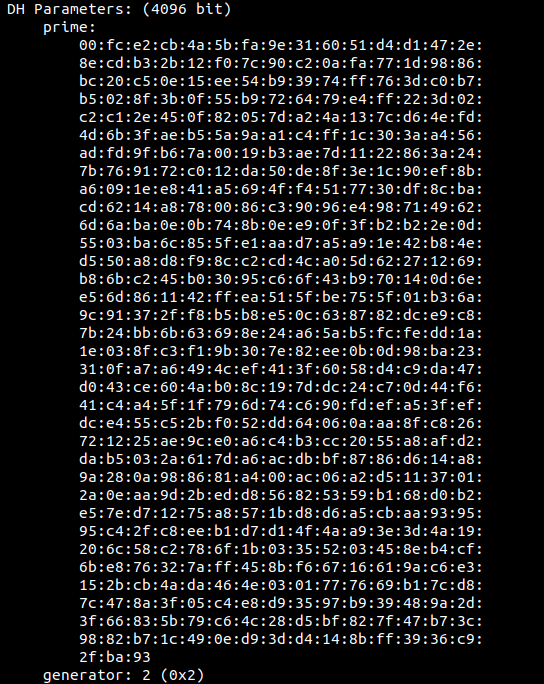
\includegraphics[width=.9\textwidth]{img/dhparam.png}
    \caption{Generation of DH parameters without the \texttt{dsaparam} option}
    \label{fig:dhparam}
\end{figure}

\section*{Exercise 2}

\begin{figure}[H]
    \centering
    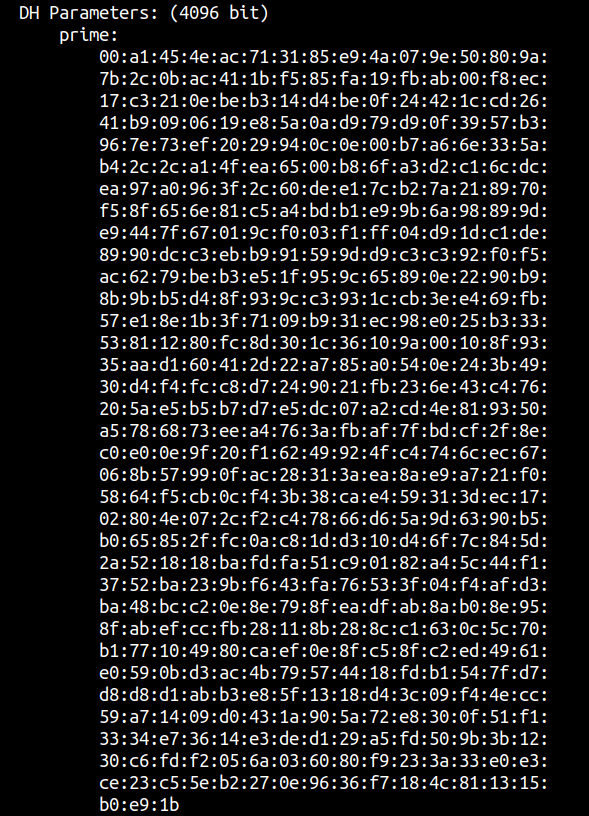
\includegraphics[width=.8\textwidth]{img/dsa-prime.png}
    \caption{Prime number generated using DH parameter generation with the \texttt{dsaparam} option}
    \label{fig:dsa-prime}
\end{figure}

\begin{figure}[H]
    \centering
    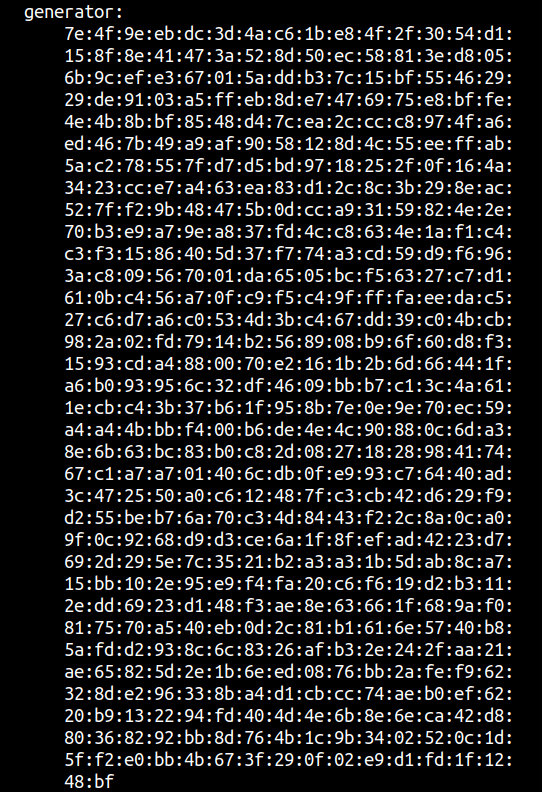
\includegraphics[width=.8\textwidth]{img/dsa-generator.png}
    \caption{Group generator generated using DH parameter generation with the \texttt{dsaparam} option}
    \label{fig:dsa-generator}
\end{figure}

\section*{Exercise 3}

\begin{figure}[H]
    \centering
    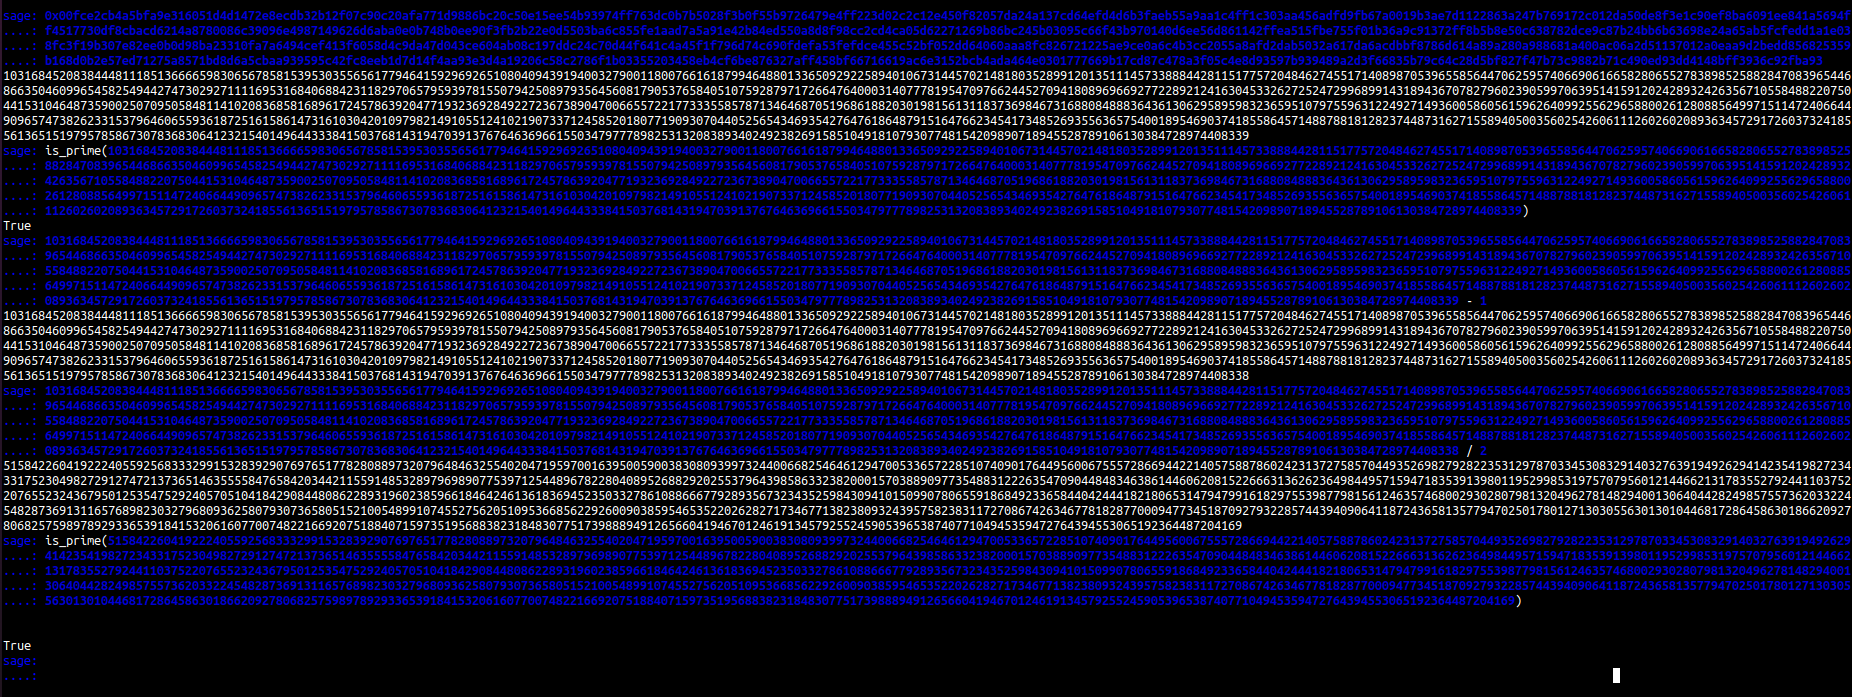
\includegraphics[width=\textwidth]{img/dh-sage.png}
    \caption{Prime number generated using DH parameter generation without the \texttt{dsaparam} option}
    \label{fig:sage-dh}
\end{figure}

\begin{figure}[H]
    \centering
    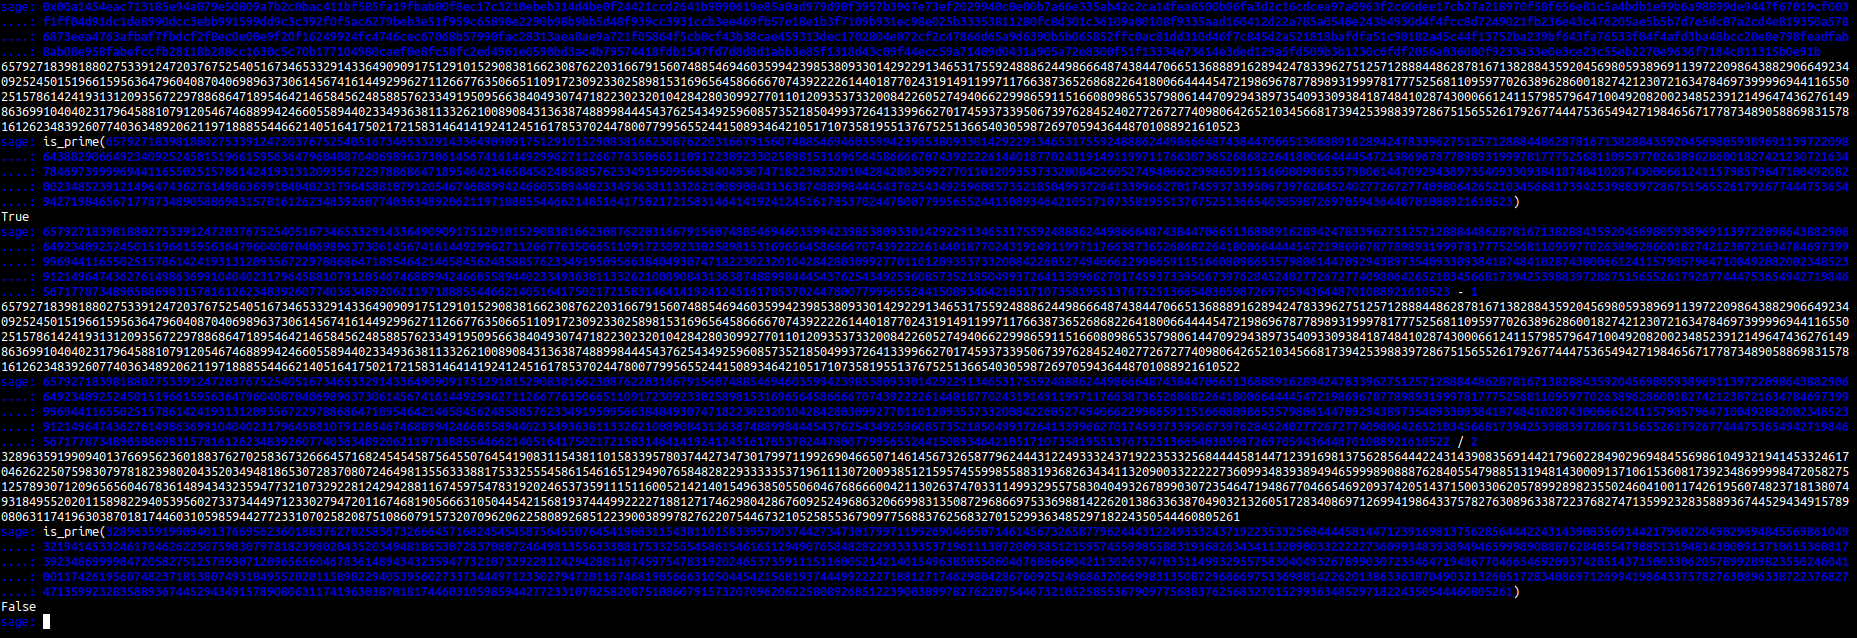
\includegraphics[width=\textwidth]{img/dsa-sage.png}
    \caption{Prime number generated using DH parameter generation with the \texttt{dsaparam} option}
    \label{fig:sage-dsa}
\end{figure}

\section*{Exercise 4}

\begin{figure}[H]
    \centering
    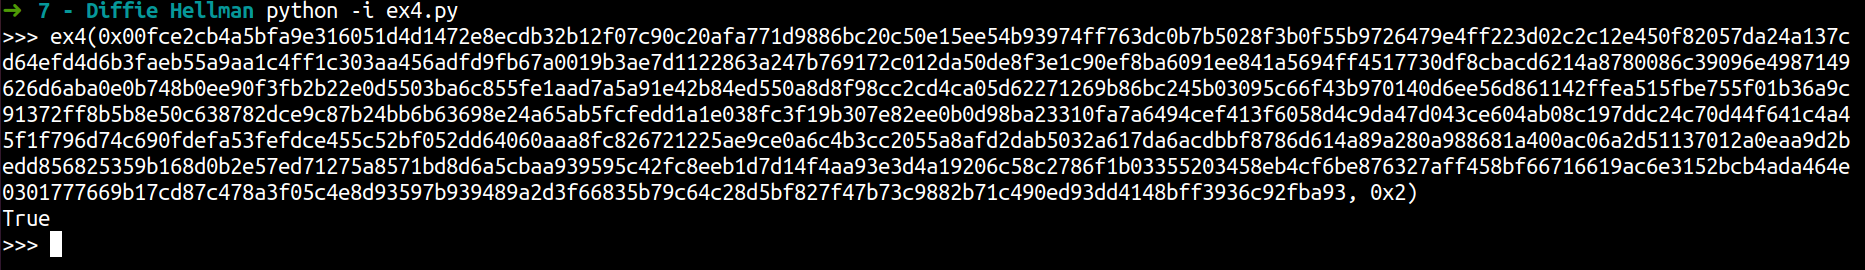
\includegraphics[width=\textwidth]{img/dh-py.png}
    \caption{Checking that $X^y \ (\mathrm{mod} \ p) = Y^x \ (\mathrm{mod} \ p)$ holds for the DH parameters generated without the \texttt{dsaparam} option}
    \label{fig:ex4-dhparam}
\end{figure}

\begin{figure}[H]
    \centering
    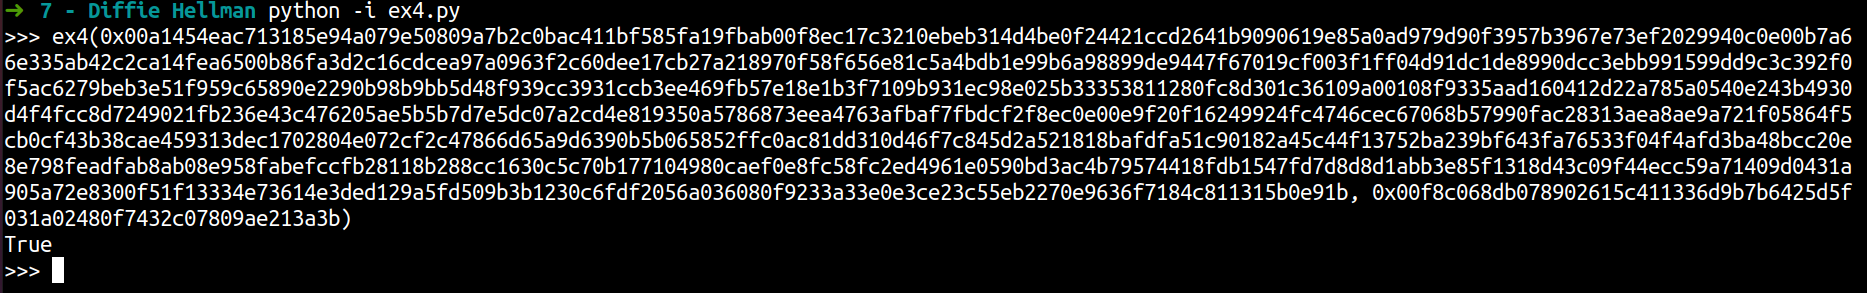
\includegraphics[width=\textwidth]{img/dsa-py.png}
    \caption{Checking that $X^y \ (\mathrm{mod} \ p) = Y^x \ (\mathrm{mod} \ p)$ holds for the DH parameters generated with the \texttt{dsaparam} option}
    \label{fig:ex4-dsa}
\end{figure}

\end{appendices}

\end{document}
